\documentclass[10pt, letterpaper]{article}
\usepackage[utf8]{inputenc}
\usepackage[spanish,es-nodecimaldot]{babel}
\usepackage[top=1in, bottom=1in, left=1in, right=1in]{geometry}

\usepackage{graphicx}
\graphicspath{{./assets/}}

\begin{document}

\begin{center}
    {\large \bfseries Modelado y Programación | Proyecto 1 \par}
    \vspace{0.2cm}
    Diego Jardón, Pablo Trinidad.
\end{center}

\section{Introducción}

A continuación se presentan los detalles del proyecto 1 del curso de Modelado y Programación
de la Facultad de Ciencias del semestre 2021-1 presentado por Diego Jardón y Pablo Trinidad.\\

Como fue descrito, el aeropuerto de la Ciudad de México tiene el requerimiento de obtener la
información del clima de vuelos que suceden a diario. Para esto nos fueron entregados dos datasets
(\texttt{dataset1.csv} y \texttt{dataset2.csv}) con información referente a algunos vuelos nacionales
e internacionales. El proyecto consta de un programa que utiliza dichos datasets para obtener la
información solicitada.\\

Se sugiere el uso de servicios web para obtener la información correspondiente del clima.

\section{Análisis del problema}

\subsection{Descripción}

Sea $A$ el universo de aeropuertos disponibles (cada aeropuerto cuenta con latitud y longitud),
y $L$ un conjunto de pares ordenados $t_i = (a, b)$ tal que $a, b \in A$ y $a$ representa
el aeropuerto de origen de un vuelo y $b$ el aeropuerto de destino, i.e:
$L = \{t_1, t_2, ..., t_n\}$. Para cada $t_1 \in L$, se busca encontrar la información meteorológica
relacionada a los aeropuertos de origen y destino de $t_i$. En particular temperatura, sensación
térmica y humedad.

\subsection{Naturaleza del problema}

Sabemos por los requerimientos del problema que $0 \leq |L| \leq 3000$, por lo que
$0 \leq |A| \leq 6000$. Sin embargo, se espera que estas ciudades estén repetidas entre los múltiples
elementos de $L$, particularmente en el dataset brindado para realizar las pruebas
(\texttt{dataset1.csv}) $|A|=X$.

\subsection{Requerimientos no funcionales}

\begin{enumerate}
  \item Se espera que las comunicación con el servicio web utilizado para obtener la información del
  clima pueda ser realizada de manera concurrente.
  \item El programa debe contar con un sistema básico de cache debe evitar realizar llamadas
  repetidas al servicio web y en su lugar utilizar las respuestas previamente obtenidas y
  almacenadas. 
\end{enumerate}

\section{Análisis y búsqueda de herramientas}
\subsection{Proveedores de información meteorológica}
\subsubsection{Requerimientos}
\subsubsection{Opciones}
\subsubsection{Comparación}
\subsection{Sistema de cache}
We used a fucking hash table mate, don't even trip.
\subsection{Llamadas concurrentes}
We used Go because ez p

Concurrency and cache model in a nutshell:
\begin{enumerate}
  \item We make all HTTP requests run in parallel
  \item Before making any HTTP request we first look up a hash table for previously fetched values (we use airport code as key), if key exists, then we don't, else, we do boiiiii.
  \item FIN.
\end{enumerate}

\begin{center}
  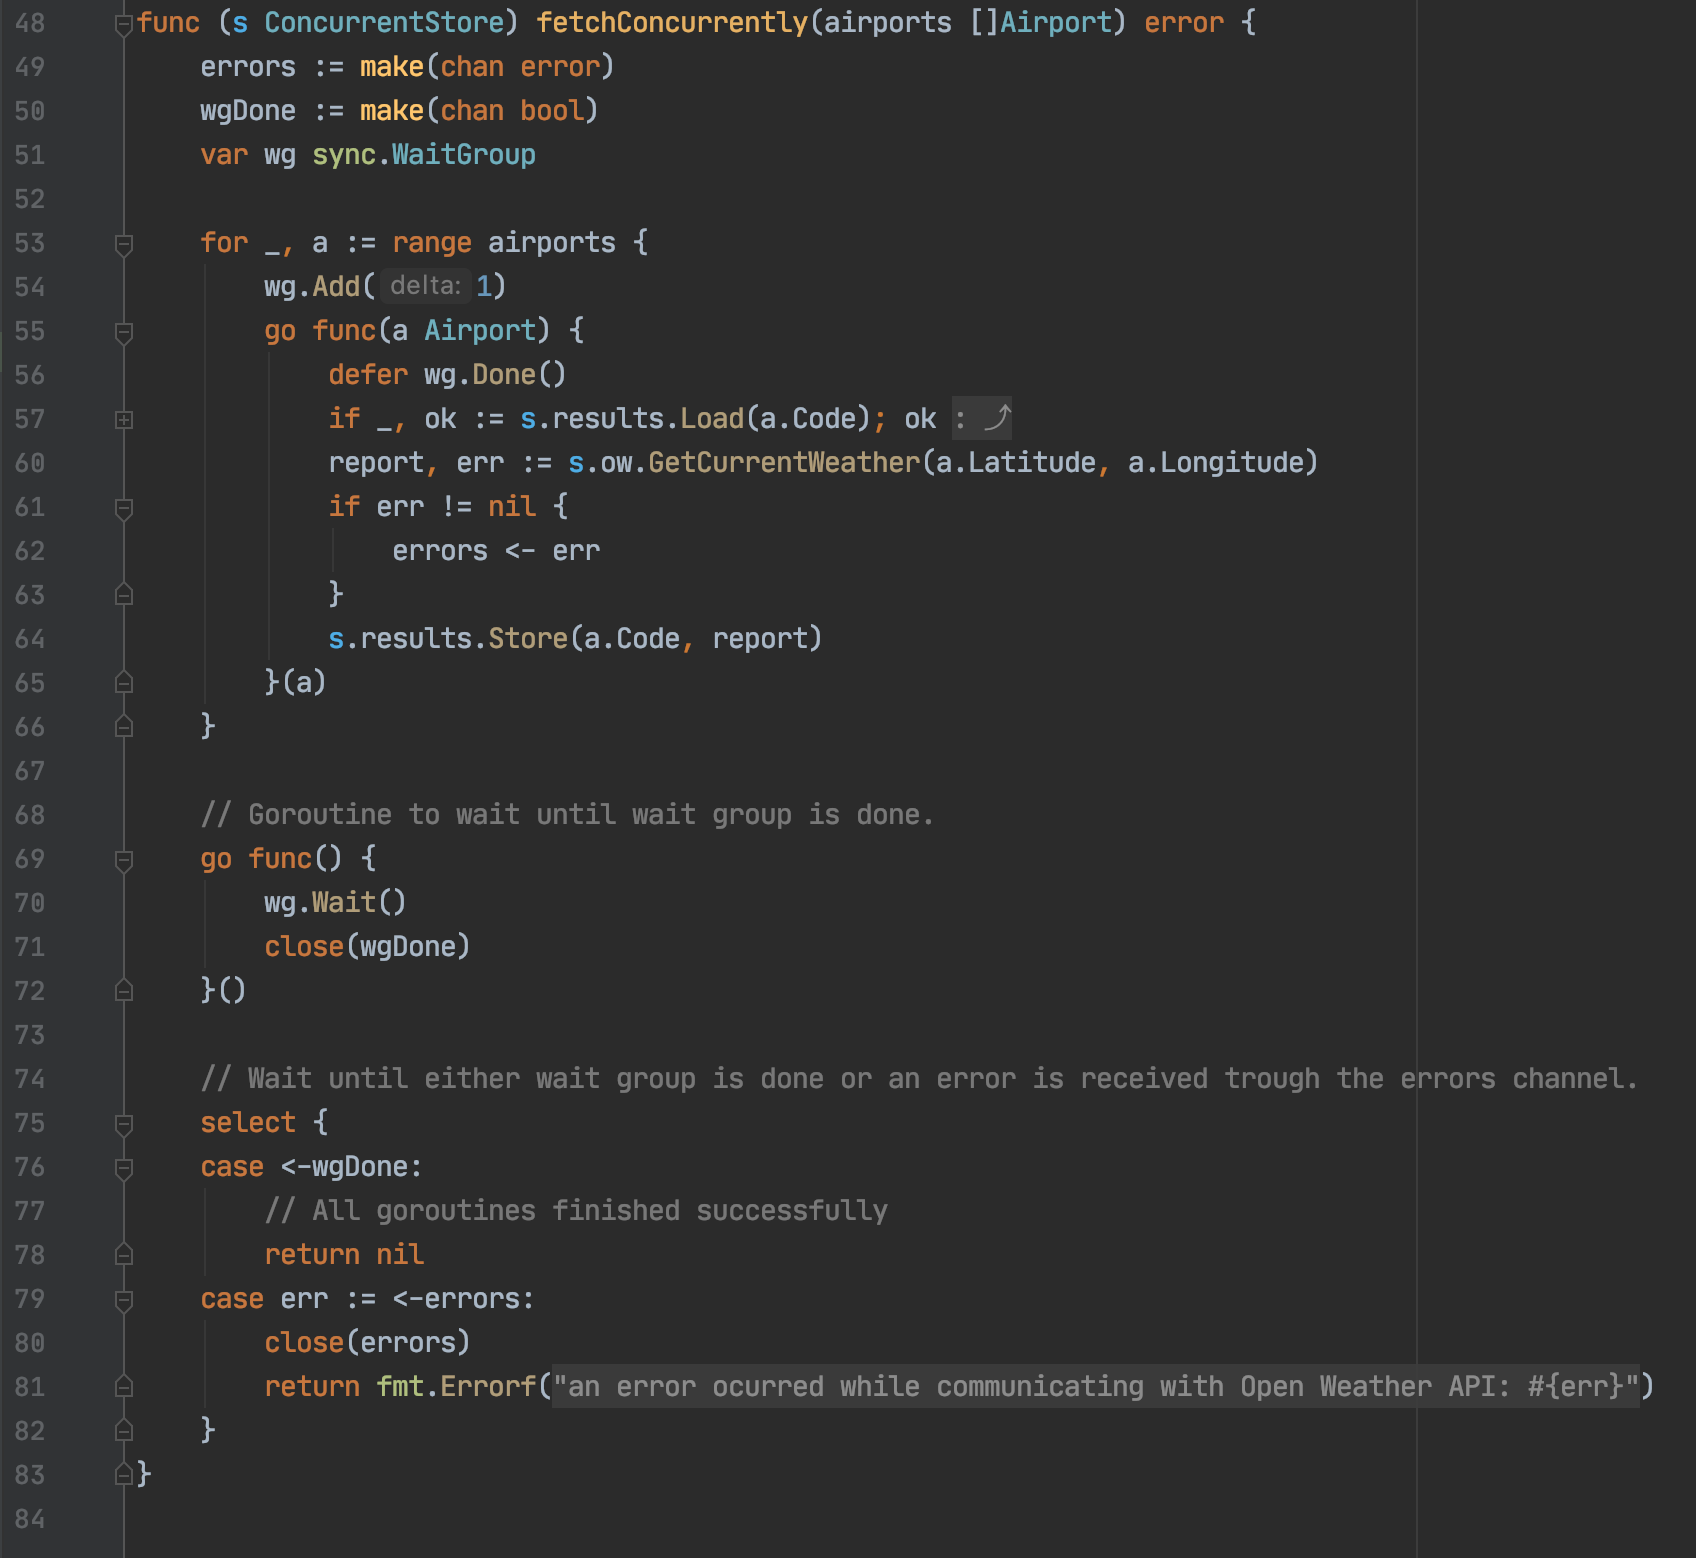
\includegraphics[scale=.4]{concurrency.png}
\end{center}

\section{Solución}
\section{Futuras mejoras}

\end{document}